\documentclass[letterpaper,11pt]{article}
\usepackage{graphicx}
\usepackage{listings}
\usepackage[super]{nth}
\usepackage[hyphens]{url}
\usepackage{hyperref}
\usepackage{amsmath}
\usepackage[makeroom]{cancel}
\usepackage[table]{xcolor}
\usepackage{comment}
\usepackage[space]{grffile}
\usepackage{csvsimple}
\usepackage{longtable}
\usepackage{adjustbox}


\newcommand*{\srcPath}{../src}%

\lstset{
	basicstyle=\footnotesize,
	breaklines=true,
}

\begin{document}

\begin{titlepage}

\begin{center}

\Huge{Assignment 4}

\Large{CS 734:  Introduction to Information Retrieval}

\Large{Fall 2017}

\Large{Grant Atkins}

\Large Finished on \today

\end{center}

\end{titlepage}

\newpage


% =================================
% First question
% =================================
\section*{1}

\subsection*{Question}

\begin{verbatim}
8.10. Consider a test collection that contains judgments 
for a large number of time-sensitive queries, such as 
"olympics" and "miss universe". Suppose that the judgments 
for these queries were made in 2002. Why is this a problem? 
How can online testing be used to alleviate the problem?
\end{verbatim}

\subsection*{Answer}

An obvious problem is that the judgements may be stale by the time new queries have been made at a later part of the day, or even a later date.
If new stories are being created and the judgements are pointing to old documents that start to become irrelevant its apparent that the judgements have to be reevaluated.
There could also be issues with bias based on the past queries.
Queries based on ``olympics'' and ``miss universe'' will have a higher relevance factor introducing bias into the results retrieved in the current state.

This is where online testing comes in.
Online testing is the idea that it is possible to test, or even train, data using live traffic.
In this problem, online testing can be used in a variety of ways based on time-sensitive queries.
Assuming there is live tracking of what queries are going out, we can track user: queries, click data, and timestamps.

There are a few ways the current system could be improved.
We can use user query timestamps to provide live updates to the relevance models that at \textit{X} time this seems like a likely query a user would ask.
The most beneficial item we can use in online testing is of course the clickthrough data based on users.
The clickthrough data will have the documents for which the user was looking for.
Although this can be difficult to integrate in live tracking, the clickthrough rate for ads or URIs provided from SERPs can help live update the documents relevance for all users.
Of course there could also be noise in the live data if everyone's click data is considered, which is unreasonable so it would probably be efficient to limit it to 10\% of the users.

%\begin{figure}[h]
%\centering
%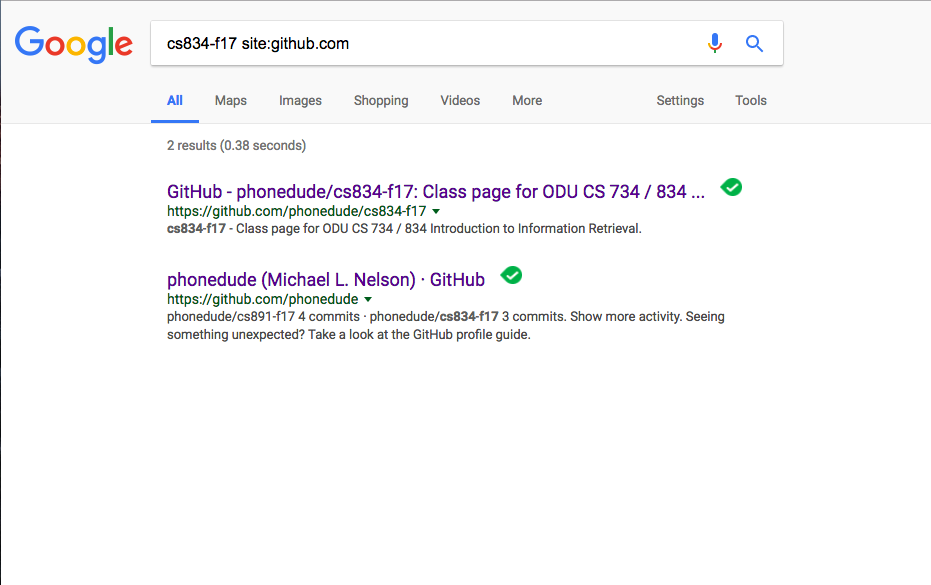
\includegraphics[scale=0.4]{sitesearch.png}
%\caption{Site search example in google}
%\label{fig:sitesearch}
%\end{figure}


\clearpage

% =================================
% Second question
% =================================

\section*{2}

\subsection*{Question}

\begin{verbatim}

\end{verbatim}

\subsection*{Answer}



\clearpage

% =================================
% 3rd question
% =================================

\section*{3}

\subsection*{Question}

\begin{verbatim}
9.8. Cluster the following set of two-dimensional 
instances into three clusters using each of the five 
agglomerative clustering methods: (-4, -2), (-3, -2),
 (-2, -2), (-1, -2), (1, -1), (1, 1), (2, 3), (3, 2), (3, 4), (4, 3)
Discuss the differences in the clusters across methods. 
Which methods produce the same clusters? How do 
these clusters compare to how you would manually
cluster the points?
\end{verbatim}

\subsection*{Answer}

To solve this problem I took I wrote a program in R named \textbf{agg\_clusters.R}, as shown in Listing \ref{lst:clust} to calculate the clusters and use the five agglomerative methods: single-linkage, average-linkage, complete-linkage, centroid-linkages, and Ward's minimum variance method.
I first created a csv file that had all the values of the 2D instances named \textbf{cluster-data.csv} located in my repository \cite{github}.
A hard lesson learned when doing this problem was that when copying and pasting from a textbook, make sure the encodings on the negative symbol are ASCII compliant or you will be left clueless.
I then read in this csv file and used the dist() method to create a matrix with the euclidean distances between each point.
From there I used the hclust() method to cluster the distance matrix for each of the agglomerative methods and created plots for each method as shown in Figures \ref{fig:1}, \ref{fig:1}, \ref{fig:3}, \ref{fig:4} and \ref{fig:5}.

To my surprise, each of the clusters/plots created were exactly the same.
I again tried using the same code, this time creating dendrograms and I was in fact getting the same clusters as shown in Figures \ref{fig:6} and \ref{fig:7}, showing dendrograms of single-linkage and complete-linkage respectively.
Compared to how I would manually cluster the points not much would change.
I would still have to find a distance metric between all of them, using euclidean, and then also I would have to compute a cost to cluster each points by.

 \lstinputlisting[frame=single,caption={R script to cluster data and create cluster plots},label=lst:clust,captionpos=b,numbers=left,showspaces=false,showstringspaces=false,basicstyle=\footnotesize]{\srcPath/agg_clusters.R}

\begin{figure}[h]
\centering
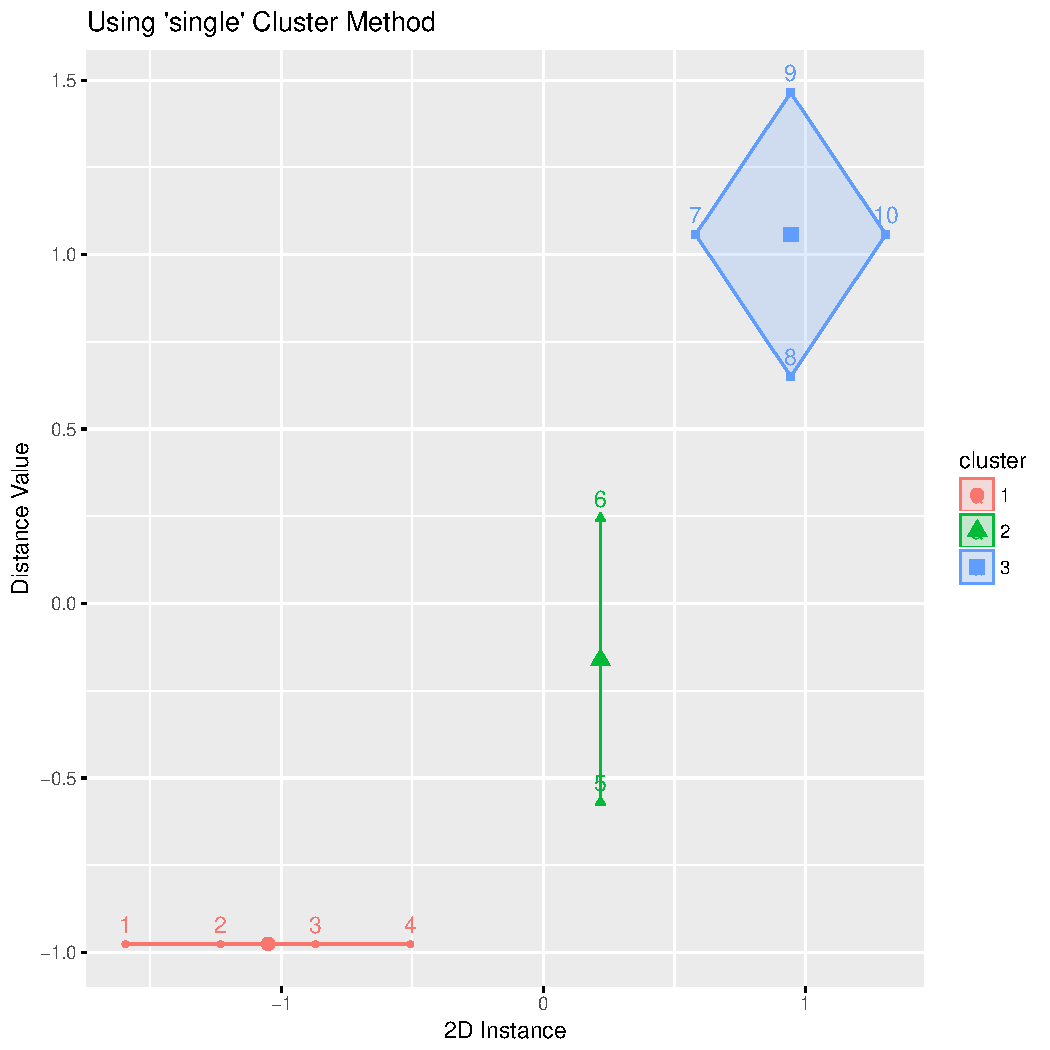
\includegraphics[scale=0.5]{single.pdf}
\caption{Single-linkage}
\label{fig:1}
\end{figure}

\begin{figure}[h]
\centering
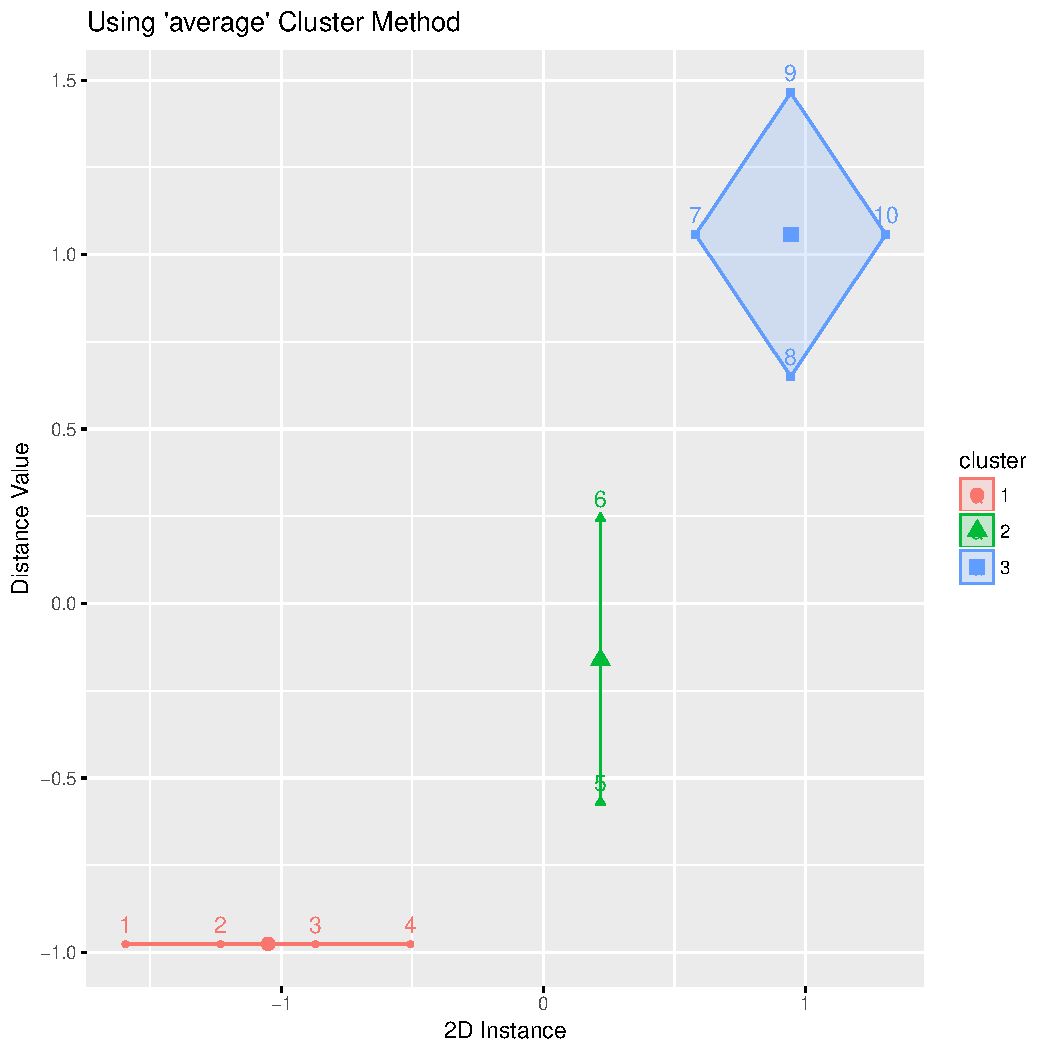
\includegraphics[scale=0.45]{average.pdf}
\caption{Average-linkage}
\label{fig:2}
\end{figure}

\begin{figure}[h]
\centering
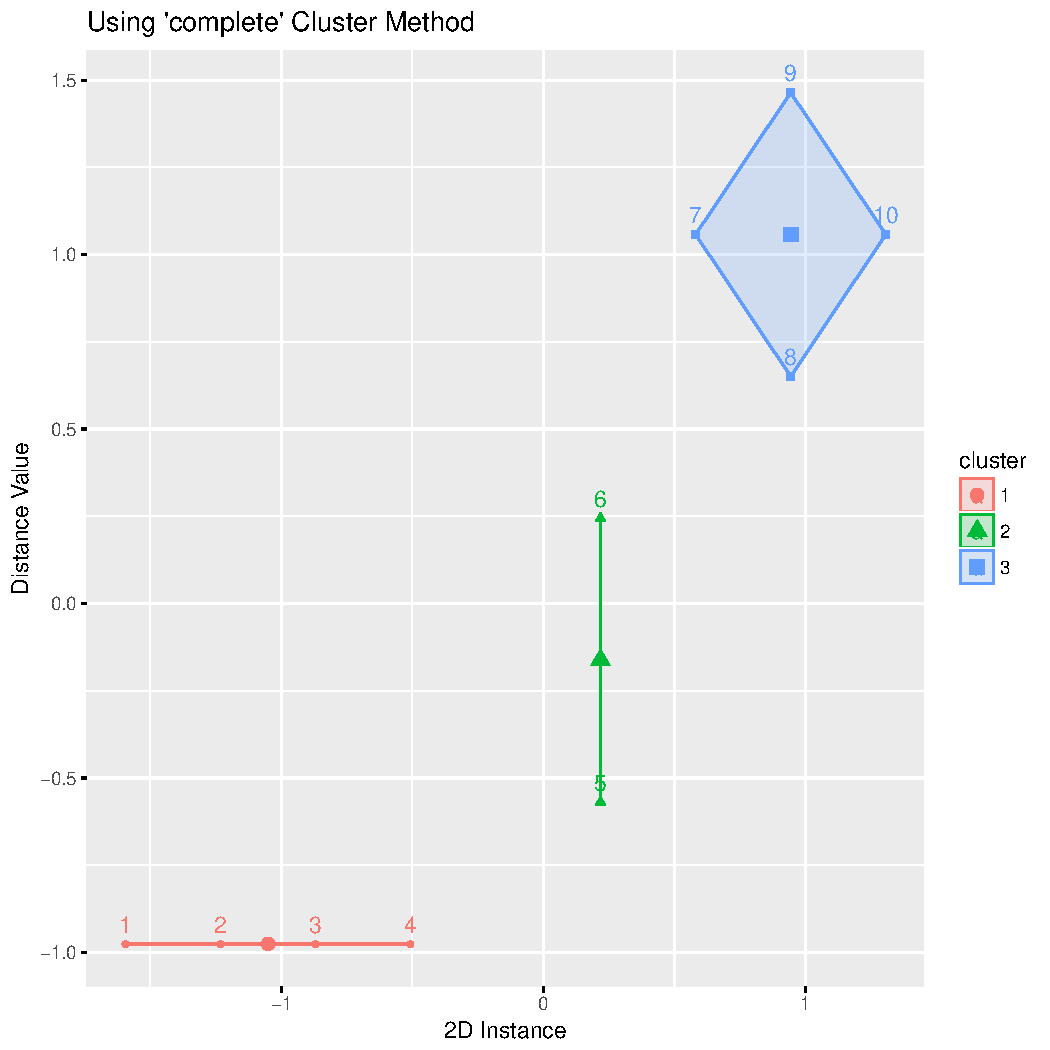
\includegraphics[scale=0.45]{complete.pdf}
\caption{Complete-linkage}
\label{fig:3}
\end{figure}

\begin{figure}[h]
\centering
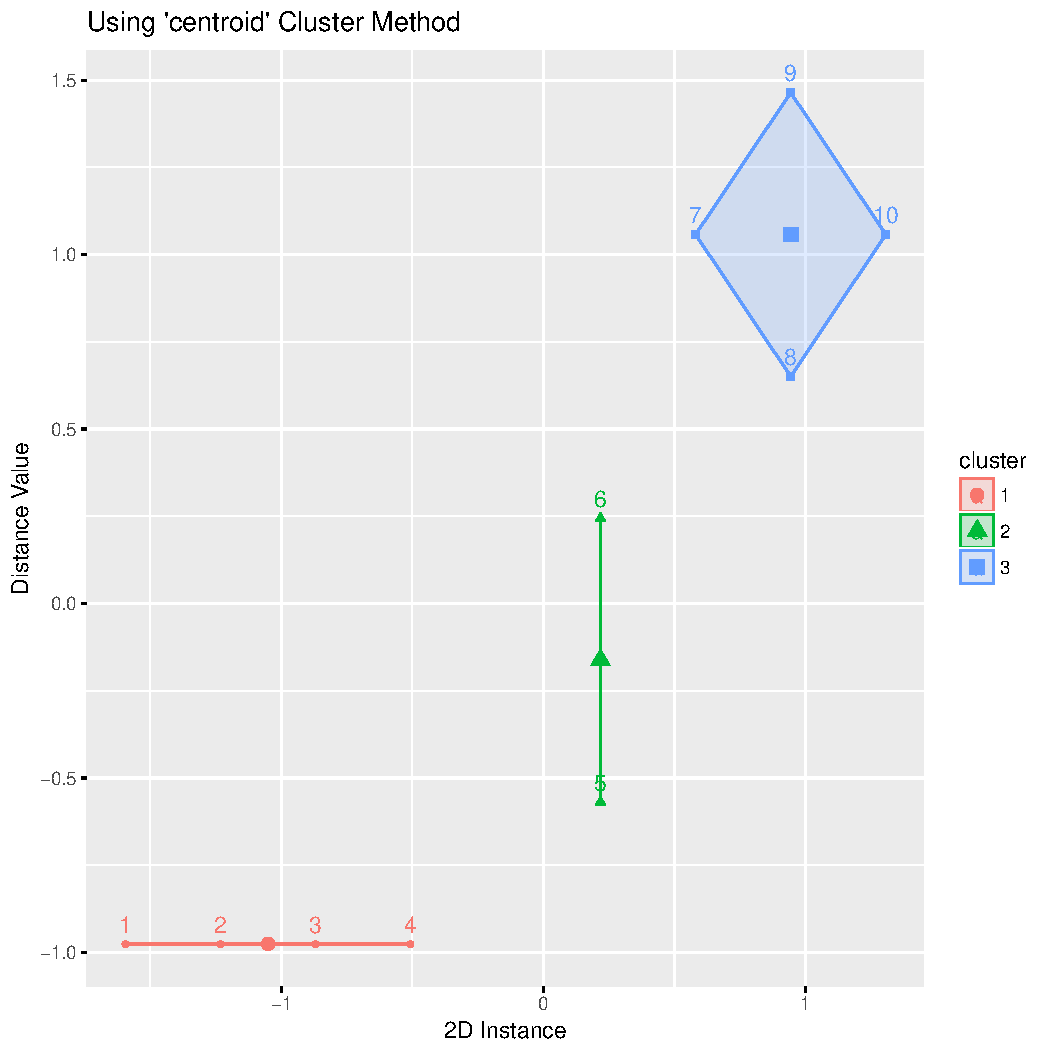
\includegraphics[scale=0.45]{centroid.pdf}
\caption{Centroid-linkage}
\label{fig:4}
\end{figure}

\begin{figure}[h]
\centering
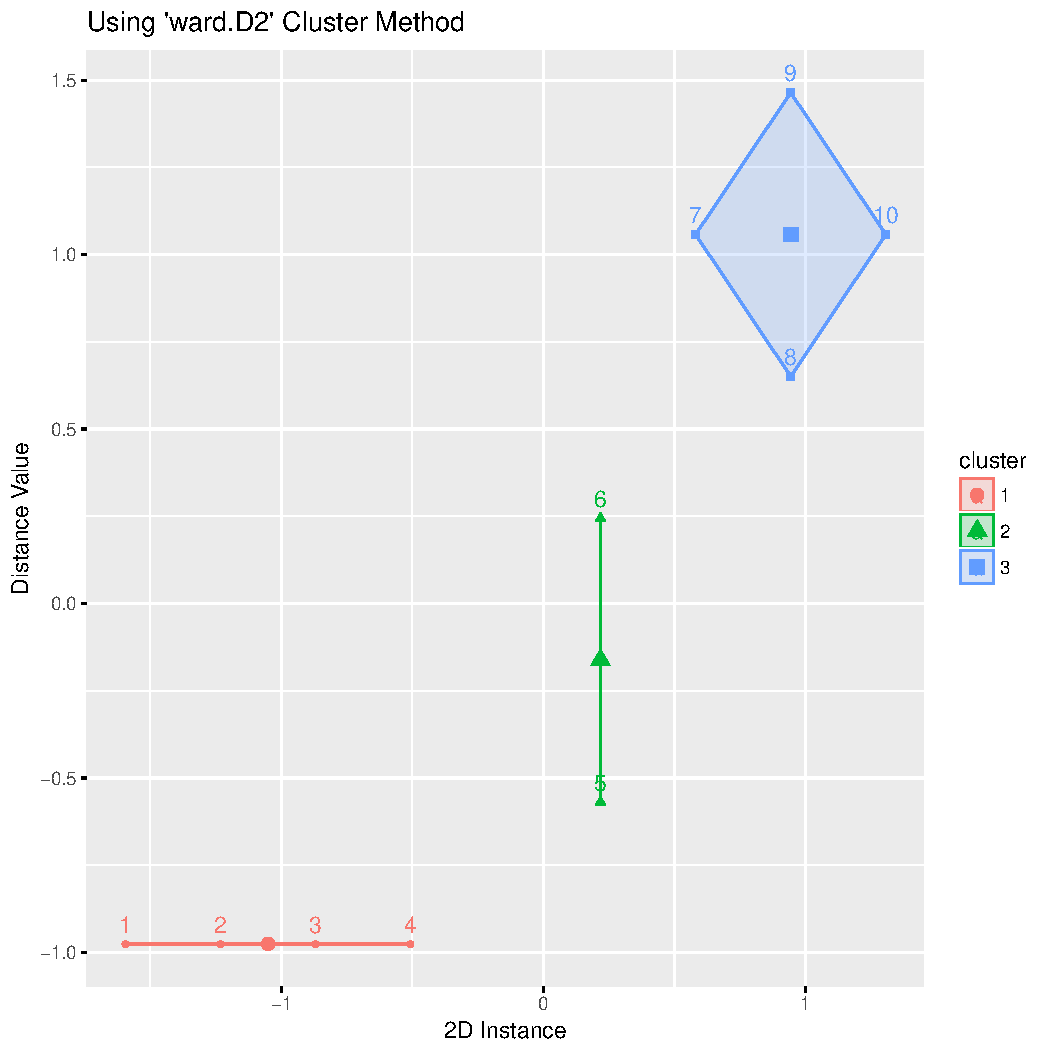
\includegraphics[scale=0.45]{ward.D2.pdf}
\caption{Ward's minimum variance method}
\label{fig:5}
\end{figure}

\begin{figure}[h]
\centering
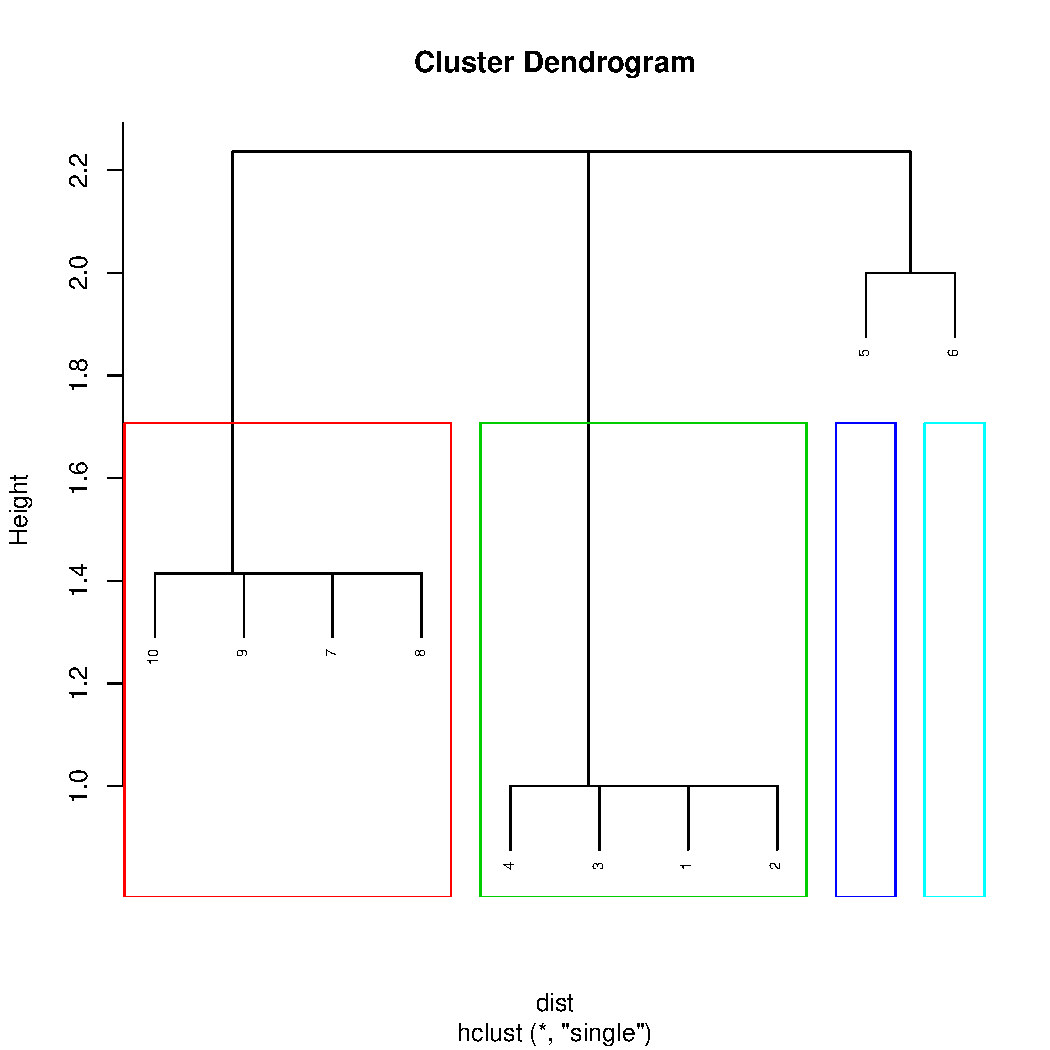
\includegraphics[scale=0.5]{single-dendro.pdf}
\caption{Single-linkage dendrogram}
\label{fig:6}
\end{figure}

\begin{figure}[h]
\centering
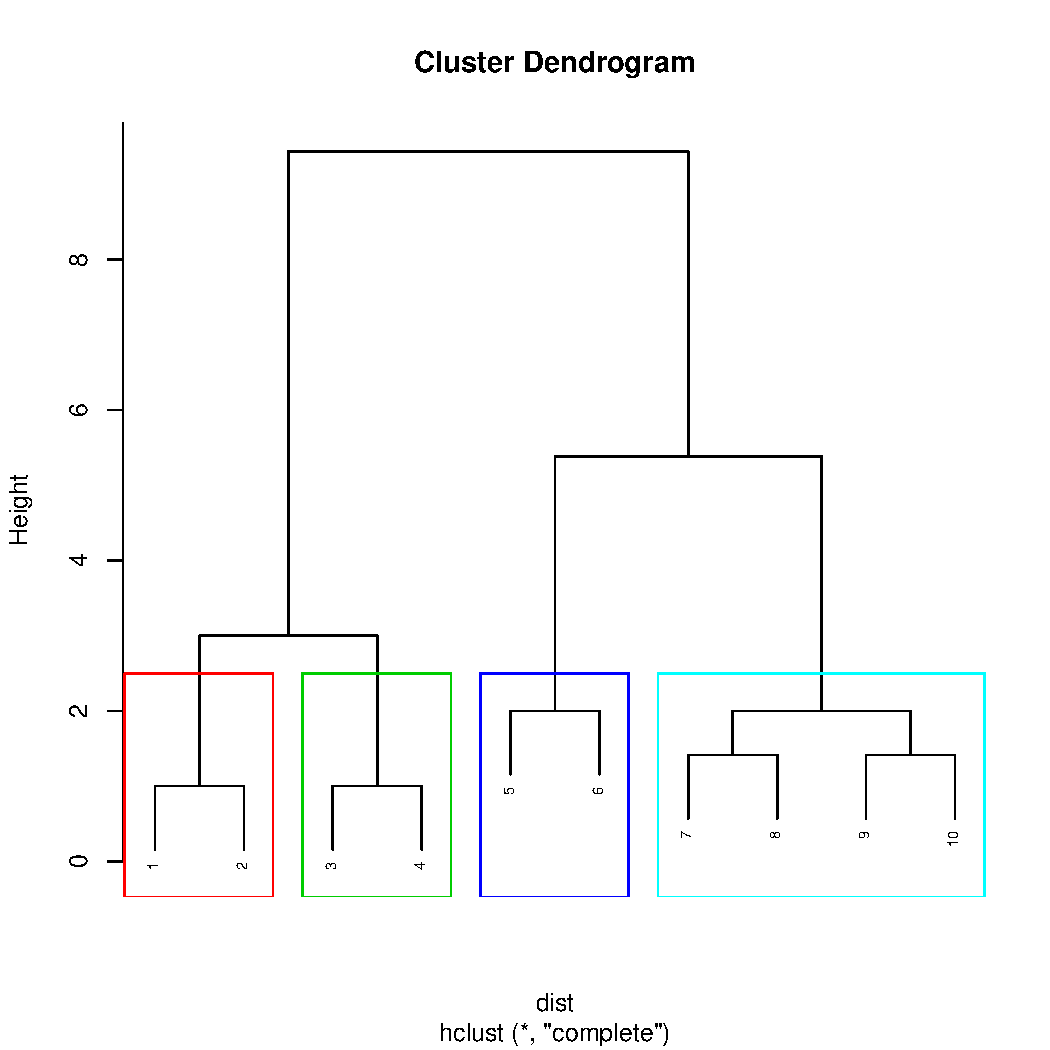
\includegraphics[scale=0.5]{complete-dendro.pdf}
\caption{Complete-linkage dendrogram}
\label{fig:7}
\end{figure}

% \lstinputlisting[frame=single,caption={Sitemap created from my assignment 1 (A1) directory},label=lst:sitemap_output,captionpos=b,numbers=left,showspaces=false,showstringspaces=false,basicstyle=\footnotesize]{\srcPath/data/sitemap.xml}

\clearpage

% =================================
% 4th question
% =================================

\section*{4}

\subsection*{Question}

\begin{verbatim}
9.9. Use K-means and spherical K-means to cluster 
the data points in Exercise 9.8. How do the clusterings 
differ?
\end{verbatim}

\subsection*{Answer}

As described in the book \cite{book}, spherical K-means is the same as K-means except that for the distance measurement between nodes is based on cosine similarity, not euclidean.
Spherical K-means seeks to get somewhat of an equal space distance between nodes.

To solve this problem I wrote an R program, as shown in Listing \ref{lst:kmeans}. 
This script utilizes the k-means function provided by the cluster library.
I first took the euclidean distance of the 2D points from 9.8, and then I also wrote a function to compute the cosine similarity in a method named \textit{cosineDist}.
After getting these two distances matrices I applied k-means to them.
The k-means clusters based on euclidean distance is shown in Figure \ref{fig:kmeans-euc}.
The k-means clusters based on cosine distance is shown in Figure \ref{fig:kmeans-cos}.

For both regular k-means and spherical k-means I specified two centers because this seemed to work out well.
Regular k-means showed to have 5 nodes in each cluster while spherical k-means showed to have a 4 to 6 split.

 \lstinputlisting[frame=single,caption={R script that computes k-means for euclidean distance and cosine similarity},label=lst:kmeans,captionpos=b,numbers=left,showspaces=false,showstringspaces=false,basicstyle=\footnotesize]{\srcPath/k_means.R}

\begin{figure}[h]
\centering
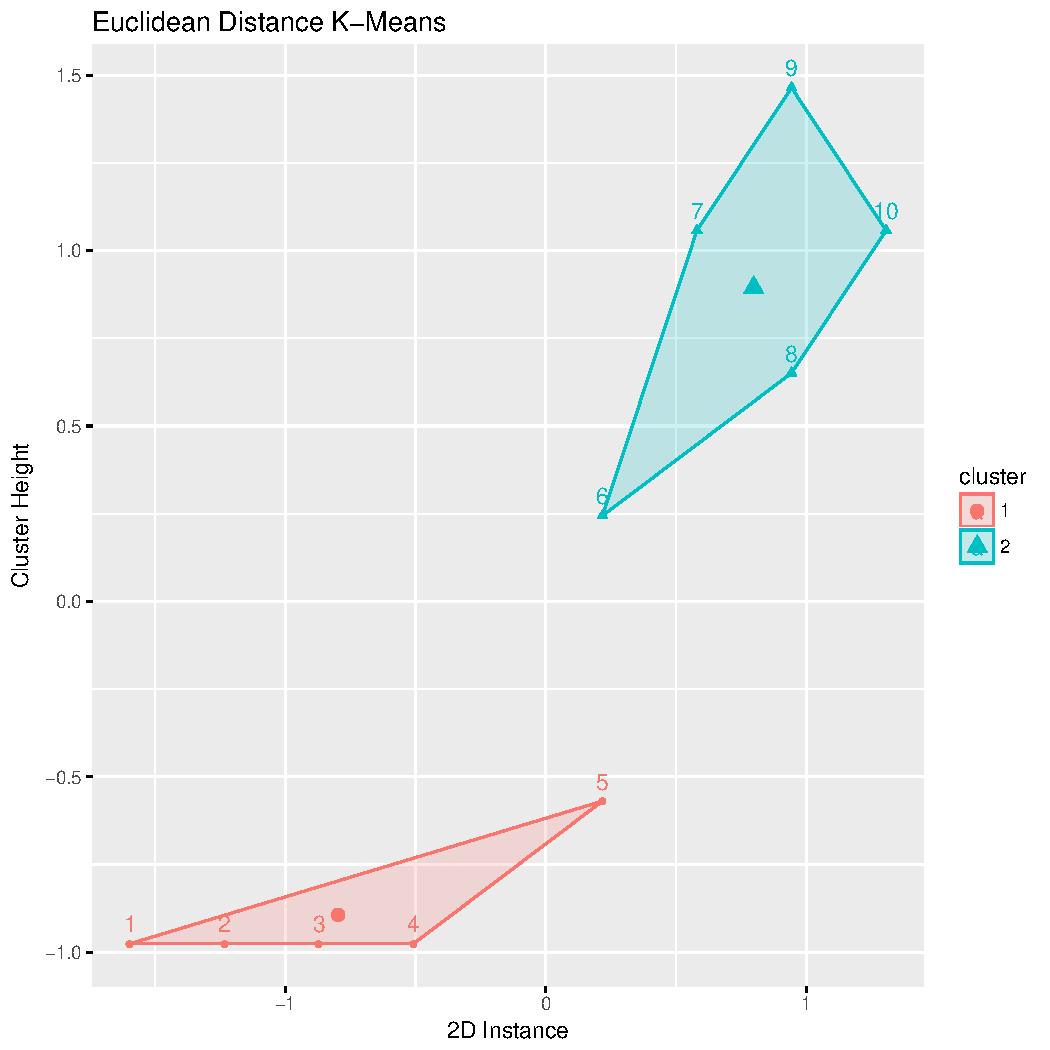
\includegraphics[scale=0.5]{kmeans-euc.pdf}
\caption{K-means with euclidean distance}
\label{fig:kmeans-euc}
\end{figure}

\begin{figure}[h]
\centering
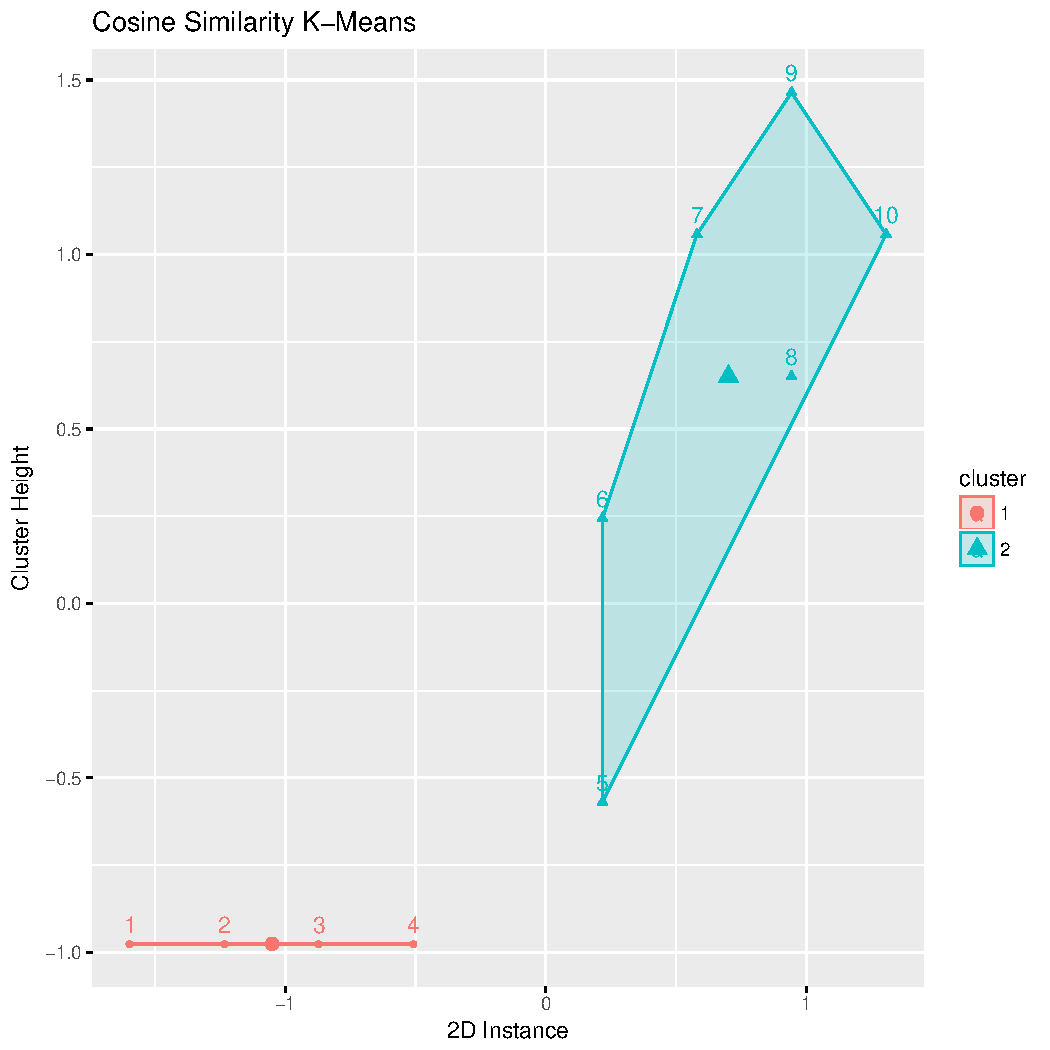
\includegraphics[scale=0.5]{kmeans-cos.pdf}
\caption{K-means with cosine distance}
\label{fig:kmeans-cos}
\end{figure}

\clearpage

% =================================
% 5th question
% =================================

\section*{5}

\subsection*{Question}

\begin{verbatim}
9.11. The K nearest neighbors of a document could be 
represented by links to those documents. Describe 
two ways this representation could be used in a search
application.
\end{verbatim}

\subsection*{Answer}

\clearpage


\clearpage


% =================================
% Bibliography
% =================================

\begin{thebibliography}{9}
\bibitem{github}
Atkins, Grant. ``CS734 Assignment 4 Repository'' Github. N.p., 4 December 2017. Web. 4 December 2017.\url{https://github.com/grantat/cs834-f17/tree/master/assignments/A4}.
\bibitem{book}
B. Croft, D. Metzler, and T. Strohman. ``Search Engines: Information Retrieval in Practice.'' Pearson, 2009. Web. 14 October 2017. ISBN 9780136072249.
\end{thebibliography}

\end{document}
